\documentclass[12pt]{article} 
\usepackage{amsmath} 
\usepackage[dvips]{graphicx}
\usepackage{multirow} 
\usepackage{geometry} 
\usepackage{pdflscape}
\usepackage[labelfont=bf]{caption} 
\usepackage{setspace}
\usepackage[running]{lineno} 
% \usepackage[numbers,sort]{natbib}
\usepackage[round]{natbib} 
\usepackage{array}
\usepackage[table]{xcolor}
\usepackage{xr}

\newcommand{\methods}{\textit{Materials \& Methods}}
\newcommand{\SI}{\textit{Appendix}~}

\topmargin -1.5cm % 0.0cm 
\oddsidemargin 0.0cm % 0.2cm 
\textwidth 6.5in
\textheight 9.0in % 21cm
\footskip 1.0cm % 1.0cm

\usepackage{authblk}

\begin{document} 

\title{Do motif roles provide unique information about species risk of extinction?\\ \medskip Supplementary Information}


\author{Anna \r{A}kesson$^{1\dagger}$, Alyssa R. Cirtwill$^{2}$, Kate Wootton$^{3}$, Gyuri Barab\'{a}s$^{1}$, Anna Ekl\"{o}f$^{1}$} 
\date{\small$^1$Department of Theoretical Biology, Chemistry, and Physics\\ 
Link\"{o}ping University\\
Link\"{o}ping, Sweden\\
\medskip
\small$^2$Department of Agricultural Sciences\\
University of Helsinki\\
Helsinki, Finland\\
\medskip
\small$^3$ University of Colorado?\\
\medskip
$^\dagger$ Corresponding author:\\
}



\maketitle 
\raggedright

\setlength{\parindent}{15pt} 
\begin{spacing}{2.0}

\clearpage

% \section*{Table of contents}
%     \begin{spacing}{1.0}

%     \begin{enumerate}
    
%         \item How do counts of motifs in a network profile vary with S and C? \\
        
%             \begin{itemize}
%             \item Same methods as main text except using counts instead of proportions to define motif profiles
%             \end{itemize}
            
            
%         \item Motif profiles differed slightly between network sets

%            \begin{itemize}
%                 \item Comparing proportions of motifs in un-filtered, filtered, and acyclic networks.
%                 \item AFAIK not referred to in text
%             \end{itemize}    
            
        
%          \item Persistence and count-based motif participation

%            \begin{itemize}
%                 \item Should be as main text section 4, but counts
%             \end{itemize}
                
        
%         \item Motif-persistence relationships and network size
%             \begin{itemize}
%                 \item Detailed results for variability of slopes for persistence $\approx$ motif participation in networks of different sizes.
%                 \item Main text refers to C, moved figure to Main while we check that we've got everything.
%             \end{itemize}


%         \item How does persistence vary with degree and trophic level?

%             \begin{itemize}
%                 \item Heat map showing persistence vs. TL with BP=0
%                 \item Heat map showing persistence vs. TL with BP=1
%             \end{itemize}
    
%     \end{enumerate}
% \end{spacing}
% \clearpage

\section{SA: Persistence and global network properties}

    Connectance and species richness had smaller effects on consumer persistence than disturbance (Figs.~\ref{fig:lm_CS}, \ref{fig:heatmap_CS}, Table~\ref{tab:per_vs_SC}).


    \begin{figure}[h!]
        \centering
        \includegraphics[width=0.95\textwidth]{figures/persistence_vs_SC_lm.eps}
        \caption{Persistence decreased strongly with increasing probability of disturbance to basal resources, while network size, connectance, and their interaction had smaller effects. \textbf{A)} Persistence decreased slightly with increasing network size at high levels of disturbance, increased slightly with increasing network size at low levels of disturbance, and did not vary noticeably with network size at moderate levels of disturbance. Networks with lower connectance (dotted line) had slightly higher persistence than networks with moderate (solid line) or high (dashed line) connectance.
        \textbf{B)} Persistence decreased with increasing connectance for all levels of disturbance and network size. Network size (line types) did not strongly affect these relationships.}
        \label{fig:lm_CS}
    \end{figure}



    \begin{figure}[h!]
      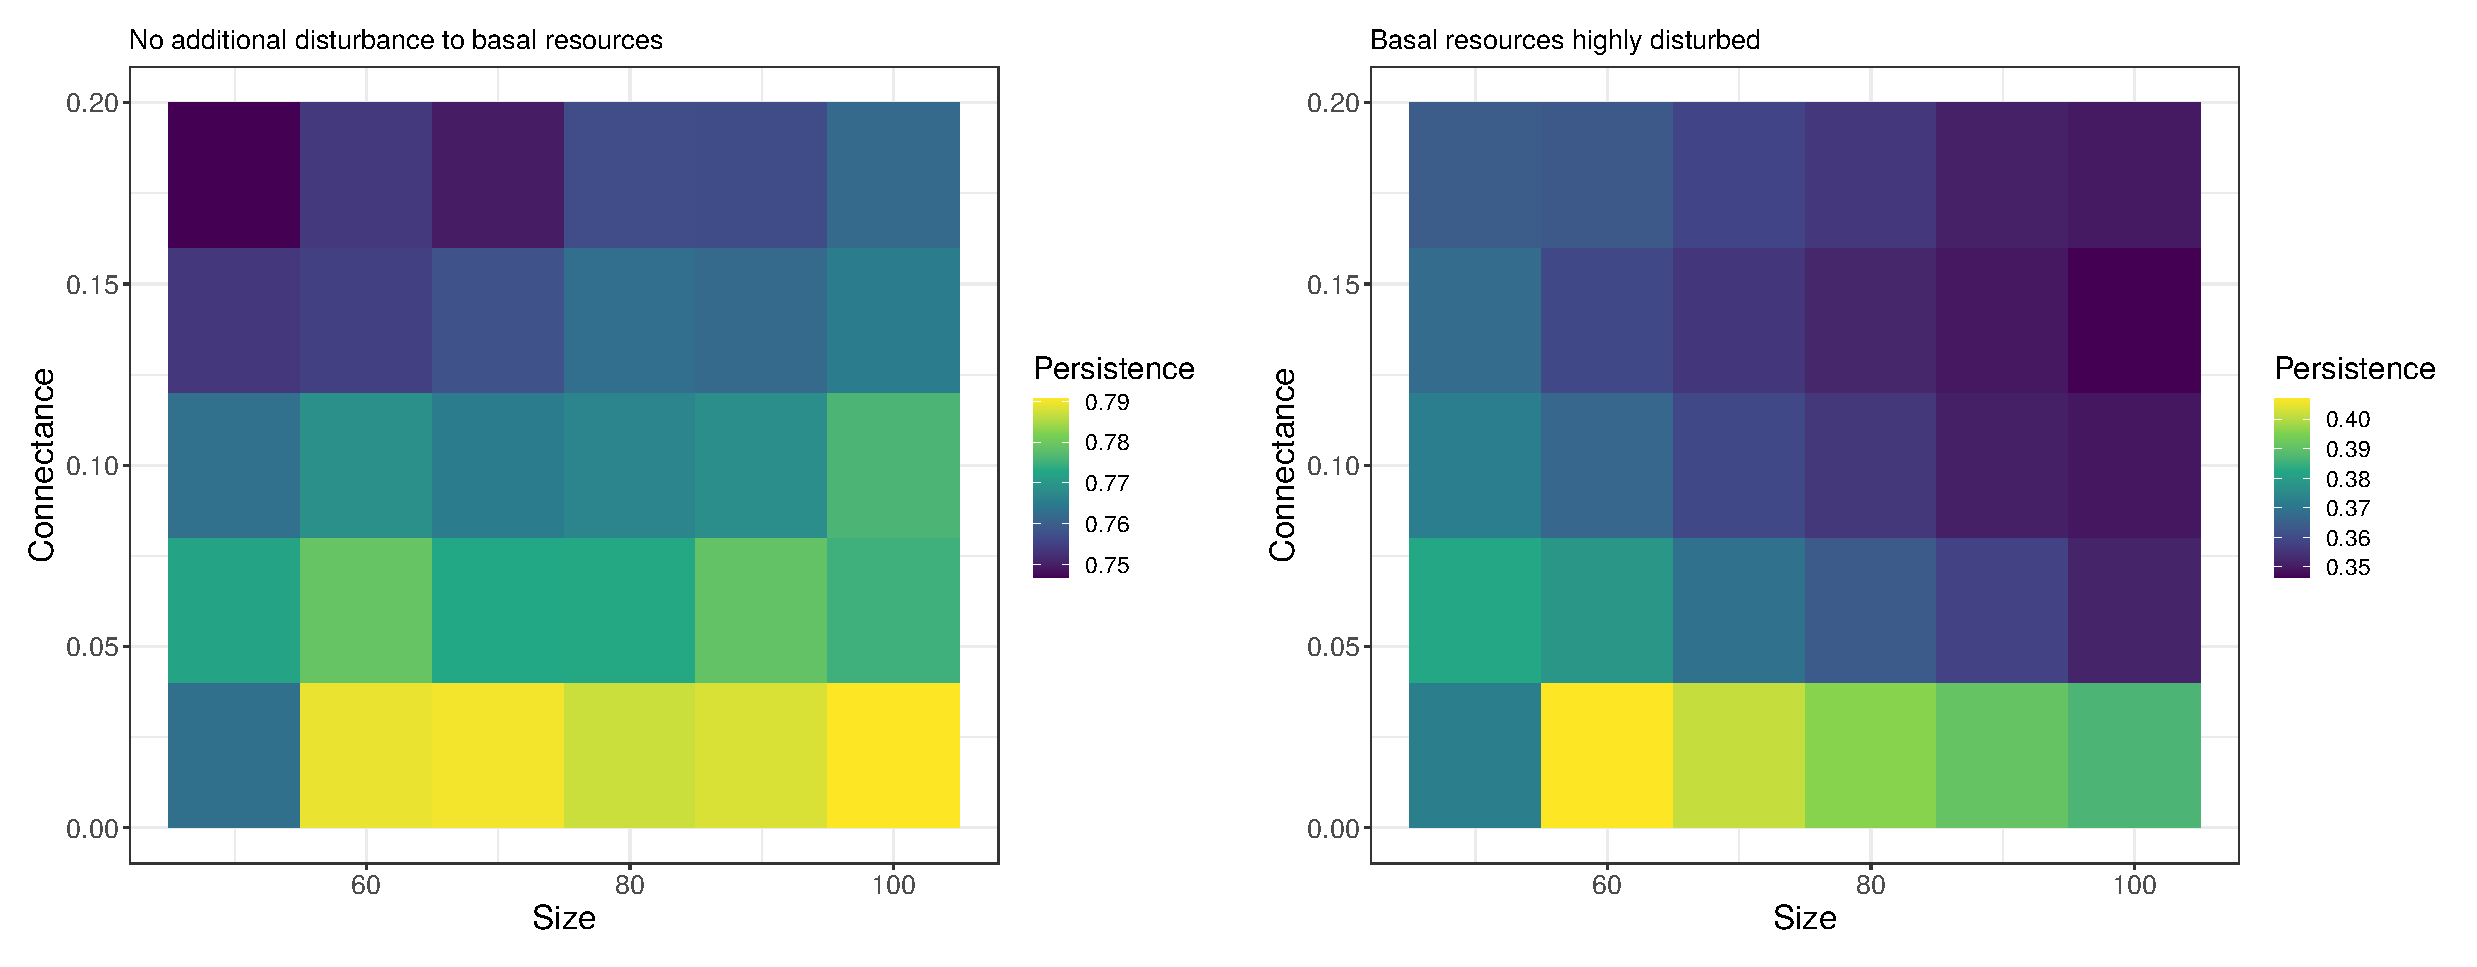
\includegraphics[width=0.95\textwidth]{figures/heatmap_CS_BPcompare.eps}
       \caption{Heat maps of average consumer persistence in networks with varying connectance (y-axis) and network size (x-axis) at two levels of disturbance to basal resources. Persistence decreases with darker color in the heat map. When basal species are not disturbed, all species experience a baseline extinction risk of $\pi = 0.1$. When basal species are highly disturbed, their baseline extinction risk rises to $\pi = 0.5$ while the baseline risk of consumers is not changed.}
       \label{fig:heatmap_CS}
    \end{figure}


    \begin{table}[hb!]
        \caption{Persistence of consumers within a network depends on network size (S) and connectance (C), the level of disturbance to basal resources (D), and interactions between them. Here we show the effect sizes ($\beta$) and $p$-values for the regression described above. All predictors were centered and scaled before fitting the model. The level of disturbance corresponds to basal resources having a probability of extinction ranging between $0.1 - 0.5$ (see \emph{Methods}).
        }
        \label{tab:per_vs_SC}
        \centering
        \begin{tabular}{c|c c |}
            Predictor & $\beta$ & $p$-value \\
            \hline
            Intercept & 0.572 & \textless0.001 \\
            Size & -5.15$\times10^{-4}$  & \textless0.001 \\
            Connectance & -0.0129 & \textless0.001 \\
            Disturbance & -0.139 & \textless0.001 \\
            S:C & -5.24$\times10^{-4}$ & \textless0.001 \\
            S:D & -3.48$\times10^{-3}$ & \textless0.001 \\
            C:D & -7.00$\times10^{-5}$ & 0.095 \\
            S:C:D: & -2.69$\times10^{-4}$ & \textless0.001 \\
        \end{tabular}
    \end{table}

\clearpage


\section{SB: Motif profiles and global properties}


    A network's normalized motif profile (i.e., proportions of the total made up by each motif) was related to the network's size, connectance, and the interaction between them ($F_{1,2996}$=74.3, $p$\textless0.001; $F_{1,2996}$=4203, $p$\textless0.001; and $F_{1,2996}$=27.8, $p$\textless0.001, respectively in a PERMANOVA of dissimilarity in normalized network motif profiles against network size, connectance, and their interaction).
    However, normalized motif profiles were not homogeneously variable across levels of network size, connectance, or their interaction  ($F_{5,2994}$=16.8, $p$\textless0.001; $F_{4,2995}$=31.7, $p$\textless0.001; and $F_{29,2970}$=11.9, $p$\textless0.001 for ANOVAs of dispersion of motif profiles against size, connectance, and combinations of size and connectance, respectively).These differences in variability can cause false positives in the PERMANOVA test. Variability was highest in small and low-connectance networks (Fig.~\ref{dispersion_normmotifs}).


   \begin{figure}[h!]
       \centering
       \includegraphics[width=.75\textwidth]{figures/proportion_profile_dispersion.eps}
       \caption{Dispersion of normalized motif profiles (i.e., proportions of each motif) within a network about the centroid for that combination of network size and connectance. Each circle represents a single network; circle colour indicates network size. Scatter has been introduced about each level of connectance to increase visual clarity; the levels of connectance we consider are indicated by vertical black lines.}
       \label{dispersion_normmotifs}
    \end{figure}


    The frequencies of the four possible motifs were related to global network properties.

    \begin{table}[hb!]
        \centering
        \caption{Coefficients for linear regressions relating the proportion of each motif in the total motif profile of a network to network size, connectance, and their interaction. Coefficients in \textbf{bold} are significant (\textless0.05).}
       \label{network_prop_lms}
       \begin{tabular}{c|c c c c c}
            Motif & Intercept & Size & Connectance & Interaction \\
            \hline
            Three-species Chain & \textbf{0.262} & \textbf{1.78$\times10^{-4}$} & \textbf{-0.157} & \textbf{-3.27$\times10^{-3}$} \\
            Apparent Competition & \textbf{0.541} & \textbf{-5.06$\times10^{-4}$} & \textbf{-1.00} & \textbf{2.59$\times10^{-3}$} \\
            Direct Competition & \textbf{0.193} & -3.56$\times10^{-5}$ & \textbf{-0.556} & \textbf{5.92$\times10^{-3}$} \\
            Omnivory & 4.82$\times10^{-3}$ & \textbf{3.64$\times10^{-4}$} & \textbf{1.71} & \textbf{-5.24$\times10^{-3}$}\\
            \hline
            \end{tabular}
    \end{table}        
\clearpage
    

\section{SC: Persistence and motif profiles}

    Persistence varied with the frequencies of different motifs in a network profile.

    
    \begin{table}[h!]
        \caption{Coefficients ($\beta$) for models relating persistence to the proportion of a network profile, the level of disturbance to basal resources (corresponding to a probability of extinction ranging between 0.1 and 0.5), and their interaction. Predictors were centered and scaled before model fitting. All effects were significant ($p$\textless0.001). We also provide the $R^2$. }
        \label{motif_profile_tab}
        \centering
        \begin{tabular}{c|c c c c c | c}
            Motif & Intercept & Proportion & Disturbance & Interaction & $R^2$\\
            \hline
            Omnivory & 0.572 & -0.0133 & -0.139 & -4.89$\times10^{-4}$ & 0.908 \\
            Apparent competition & 0.572 & 0.0105 & -0.139 & 4.78$\times10^{-4}$ & 0.905 \\
            Direct competition & 0.572 & 2.62$\times10^{-3}$ & -0.139 & 3.84$\times10^{-4}$ & 0.901 \\
            Three-species chain & 0.572 & 6.12$\times10^{-3}$ & -0.139 & -1.90$\times10^{-4}$ & 0.901 \\ 
        \end{tabular}
    \end{table}


\clearpage


\section{SD: Persistence and motif participation}

    Persistence varied with motif participation.

    
    \begin{table}[h!]
        \centering
        \caption{Coefficients ($\beta$) and $p$-values ($p$) for models relating persistence to the proportion of a species' role made up by the focal motif, the level of disturbance to basal resources (corresponding to a probability of extinction ranging between 0.1 and 0.5), and their interaction, as well as a random intercept to account for differences in persistence across levels of network size and connectance (Equation~\ref{propreq}). Predictors were centered and scaled before model fitting. We also provide the marginal $R^2_M$ (fixed effects only) and conditional $R^2_C$ (fixed and random effects) for each model.}
        \label{tab:proportion}                \footnotesize
        \begin{tabular}{c|c c | c c | c c | c c | c c |}
        & \multicolumn{2}{c|}{Intercept} & \multicolumn{2}{c|}{Proportion} & \multicolumn{2}{c|}{Disturbance} & \multicolumn{2}{c|}{Interaction} & \multicolumn{2}{c|}{$R^2$} \\
        Motif & $\beta$ & $p$ & $\beta$ & $p$ & $\beta$ & $p$ & $\beta$ & $p$ & $R^2_M$ & $R^2_C$ \\
        \hline
        3-sp Chain & 0.574 & \textless0.001 & -0.00508 & \textless0.001 & -0.139 & \textless0.001 & -0.00337 & \textless0.001 & 0.900 & 0.912 \\
        App. Com. & 0.574 & \textless0.001 & -0.00312 & \textless0.001 & -0.139 & \textless0.001 & 0.00410 & \textless0.001 & 0.900 & 0.911 \\
        Dir. Com. & 0.574 & \textless0.001 & 0.00564 & \textless0.001 & -0.139 & \textless0.001 & 0.000256 & \textless0.001 & 0.901 & 0.911 \\
        Omnivory & 0.574 & \textless0.001 & 0.00709 & \textless0.001 & -0.139 & \textless0.001 & -0.00198 & \textless0.001 & 0.894 & 0.912 \\
        \end{tabular}
    \end{table}        
\clearpage     


\section{SE: Motif-persistence relationships \& network size}

    When comparing the outcomes from linear mixed-effect models (LMMs) relating persistence to motif roles across all networks (Fig. 3 and Table 1, \emph{Main Text}) with similar linear regressions (LRs) made on each single network separately, the main trends are similar but different-sized networks showed slightly different results results for some motifs (Figure temporarily in main text).%(Figure~\ref{fig:density_prop_S}). 
    For the three-species chain and omnivory motifs, a significant interaction between disturbance and the effect of the focal motif means that having a larger proportion of the role be made up of the chain or omnivory motif is associated with lower persistence at high levels of disturbance (Fig. 3 and Table 1, \emph{Main Text}). 
    The same pattern holds overall for LRs fit within a network  %(Figure~\ref{fig:density_prop_S})
    : the fraction of negative slopes for the proportion of three-species chain and omnivory motifs increases with increasing disturbance. 
    This trend is most pronounced in large networks.% (bottom panel, Figure~\ref{fig:density_prop_S}). 
    Besides the decrease in fraction of positive slopes with increasing disturbance, the omnivory motif show a higher overall fraction of positive slopes in comparison to the three-species chain motif, corresponding to the positive main effect of omnivory (Fig. 3 and Table 1, \emph{Main Text}). 


    \begin{figure}[h!]
         \centering
         % 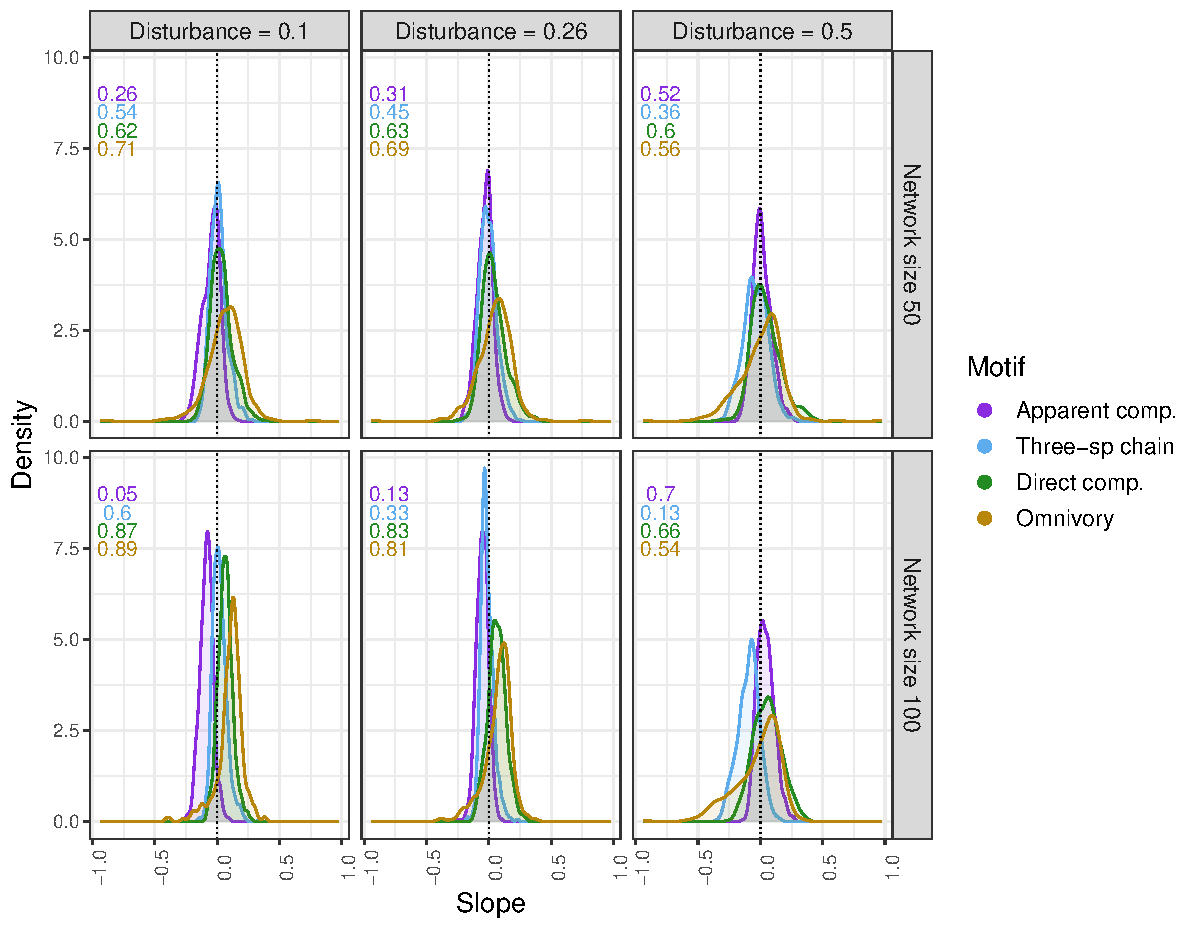
\includegraphics[width=\textwidth]{figures/prop_dens_bp_vs_S_allC.pdf}
        \caption{Density (y-axis) of slopes (x-axis) for all simulated webs of all sizes - a visualization of how an increased proportion of each motif (different colored lines) affects persistence of consumer species. The slopes are derived from linear mixed-effect models, with a random intercept for the interaction between species richness and network size. A negative slope value reflects a negative relationship between increased participation in a motif and persistence, while a positive slope value reflects a positive relationship - an increased proportion of a specific motif increase persistence. The fraction of replicates with a slope greater than zero are stated in numbers in each sub-plot, the color corresponding to motif (legend). Columns show the result for various disturbances on the basal level, from $\pi_{disturbed} = 0.1$ (left) to $\pi_{disturbed} = 0.5$ (right). Rows show various levels of network size. The vertical line indicate zero on the x-axis.}
        \label{fig:density_prop_S}
    \end{figure}
    
    
    For the apparent and direct competition motifs, the LMMs include a positive interaction between disturbance and the proportion of the motif in a species' role (Fig. 3 and Table 1; \emph{Main Text}).
    This means that having more of the role made up of these two motifs is increasingly beneficial at higher levels of disturbance, a trend which is also evident from the increasing fraction of positive slopes with increasing disturbance based on LRs of each network at each level of disturbance. % (Figure~\ref{fig:density_prop_S}).
    As with the trends for omnivory and three-species chains, these increases are strongest in large networks. % (bottom row, Figure~\ref{fig:density_prop_S}).
    % For direct competition, the fraction of slopes are similar across disturbance levels. Although this interaction is not positive when accounting for network size, the fraction of positive slopes are throughout high.
    The increase in the proportion of positive slopes was much stronger for apparent competition than direct competition, consistent with the smaller (but still significant) interaction term for between direct competition in the LMMs.
    A high proportion of direct competition in a species' role tended to be associated with greater probability of persistence across levels of disturbance and network size.
    % In conclusion, species richness does not considerably alter the trends visible in the LMMs. High species richness more clearly display an interaction between motif proportion, persistences and disturbance levels, while this effect is smaller with low species richness. 
\clearpage
                
            
\section{SF: Persistence, degree, and trophic level}


    Persistence varies with in-degree, trophic level, and their interaction.

    \begin{table}[h!]
        \caption{Coeffcients ($\beta$) for regressions of consumers' probabilities of persistence against simple measures of species' role (STL or in-degree), level of disturbance to basal resources, and their interaction. Predictors were centered and scaled before model fitting. All $p$-values were \textless0.001. The level of disturbance is reflected by basal resources having a baseline probability of extinction ranging between $0.1 - 0.5$.}
        \label{tab:per_vs_TLdeg}
        \centering
        \begin{tabular}{l|c  c  c |}
            Simple role measure & Role & Disturbance & Interaction \\
            \hline
            STL & -0.0218 & -0.139 & 0.00508 \\
            in-degree & -0.00130 & -0.139 & -0.00908 \\
        \end{tabular}
    \end{table}


    \begin{figure}[h!]
     \centering
     % 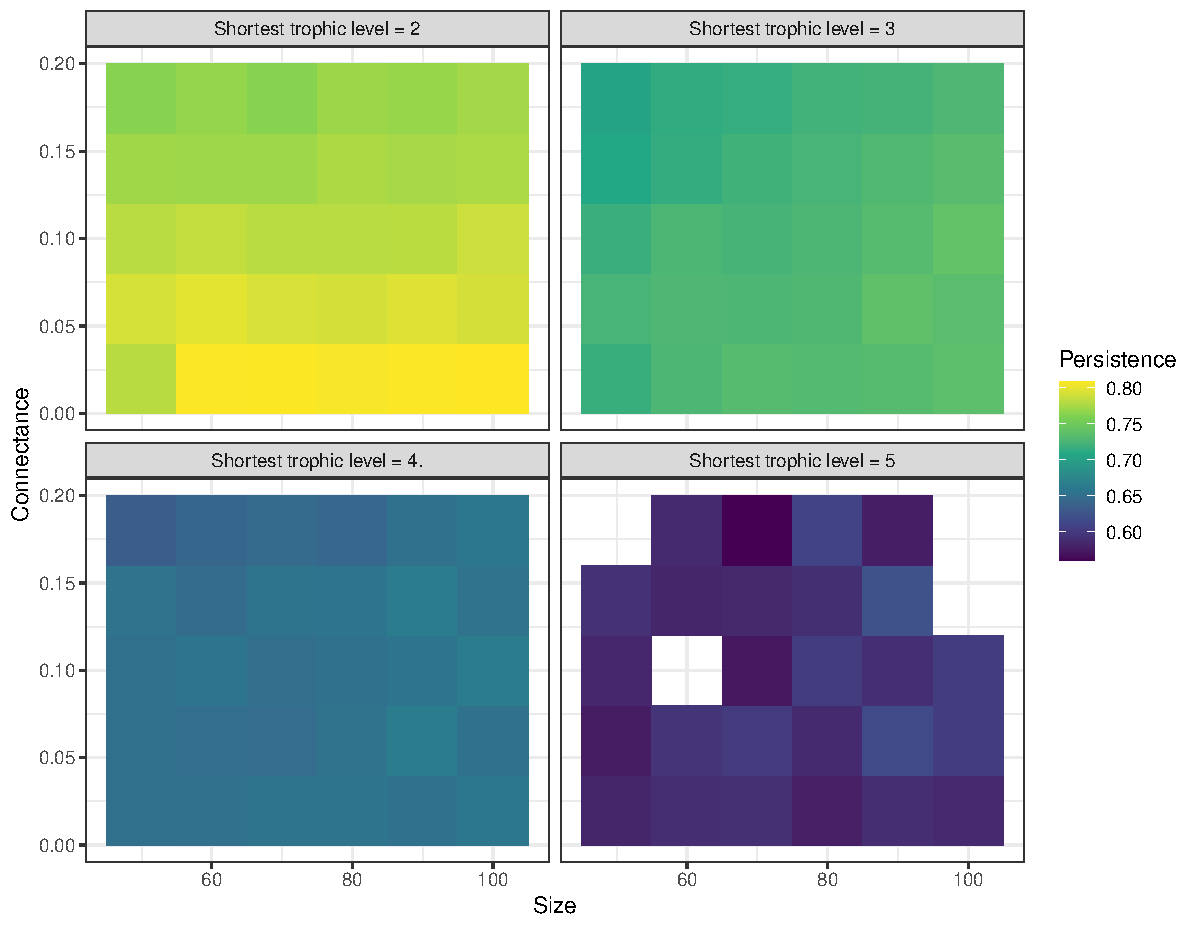
\includegraphics[width=0.8\textwidth]{figures/heatmap_STL_allCS_BP0.pdf}
     \caption{All species across all levels experience a risk of going extinct due to causes not related to the web of $\pi = 0.1$. The sub figures show final persistence for consumers with different shortest trophic length, for increasing connectance (y-axis) and network size (x-axis). Persistence decreases with darker color in the heat map.}
     \label{fig:heatmap_stl_BP0}
    \end{figure}


    \begin{figure}[h!]
     \centering
     % 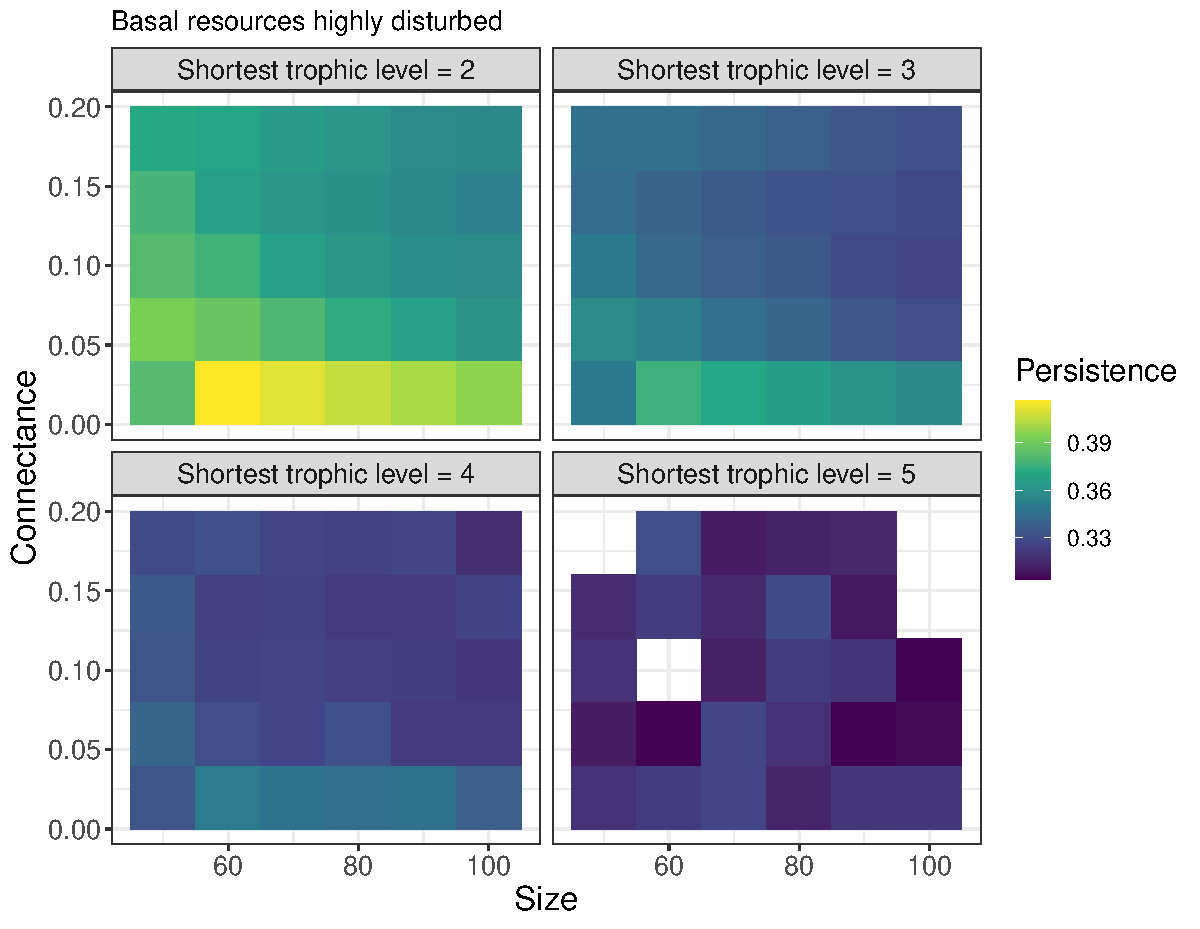
\includegraphics[width=0.8\textwidth]{figures/heatmap_STL_allCS_BP1.pdf}
     \caption{Primary producers experience a disturbance reducing their probability to go extinct to $\pi_{disturbed} = 0.5$ All consumer species go extinct due to causes not related to the web itself with probability $\pi = 0.1$. The sub figures show final persistence for consumers with different shortest trophic length, for increasing connectance (y-axis) and network size (x-axis). Persistence decreases with darker color in the heat map.}
     \label{fig:heatmap_stl_BP1}
    \end{figure}

\clearpage

\section{SG: Motif participation and network properties}


    Motif participation varies with global-scale network properies.

    \begin{table}[hb!]
        \centering
        \caption{Motif participation varies with size and connectance. Here we give the range and mean ($\pm$ standard deviation) proportion of each motif in species' motif participation vectors. 
        We also show the effects ($\beta$) of network size, connectance, and their interaction in linear models predicting the proportion of each motif in a participation vector.
        All effects were significant ($p$\textless0.001).
        Predictors were not centered or standardized before model fitting. Motifs are ordered according to mean proportion.}
        % Relevant lms are pchainlm, pomnilm, papplm, pdirlm}
        \label{tab:partic_vs_SC}   
        \footnotesize
        \begin{tabular}{c|c c c | c c c}
            Motif & Min & Max & Mean (SD) & Size & Connectance & Interaction \\
            \hline
            3-sp Chain & 0 & 1 & 0.249 (0.127) & 2.22$\times10^{-4}$ & -0.131 & -3.20$\times10^{-3}$ \\
            App. Comp & 0.250 & 0.765 & 0.422 (0.0645) & -5.06$\times10^{-4}$ & -1.00 & 2.59$\times10^{-3}$ \\
            Dir. Comp & 0.0501 & 0.359 & 0.179 (0.0407) & -3.56$\times10^{-5}$ & -0.556 & 5.92$\times10^{-3}$ \\
            Omnivory & 0.006 & 0.346 & 0.164 (0.0790) & 3.64$\times10^{-4}$ & 1.71 & -5.24$\times10^{-3}$ \\   
            \hline
            \end{tabular}
            \end{table}


    \begin{figure}[h!]
        \centering
        \includegraphics[height=.65\textheight]{figures/participation_vs_SC.eps}
        \caption{The proportion of each motif in a consumer's participation vector varied with network size, connectance, and their interaction. These relationships were steepest for apparent competition and omnivory.}
        \label{fig:roles_vs_SC}
    \end{figure}
\clearpage 

\section{SH: Persistence and motif roles}

    \subsection*{Methods}

        As one more level of detail, we can consider the frequency with which a species appears in each \emph{position} in each motif. 
        Different positions are associated with different numbers of predators and prey, making the similarities and differences between motifs and degree more explicit.
        The full set of these positions, across all motifs, is the species' \emph{motif role}~\citep{Stouffer2010,Cirtwill2017}.
        As with motif participation, we normalized motif roles by dividing the number of times a species appeared in each position by the total number of times it appeared in all positions~\citep{Baker2015,Cirtwill2017}.
        
        
        [[Could add a PERMANOVA to show that species' roles overal affect their persistence. Haven't done so yet.]]
        

        To test whether participating in different motif positions was related to a species' probability of persistence, we fit similar models to those for motif participation.
        For each position, we fit a linear mixed-effect model relating persistence to the frequency of the position in a species' motif role, disturbance, and their interaction.
        To account for differences in persistence across networks of different size and connectance, we included a random effect of the interaction between size and connectance.
        All regressions were fit using the R~\citep{R} function `lmer' from the package \emph{lmerTest}~\citep{lmerTest}.

    
    \subsection*{Results}

    \begin{table}[h!]
        \caption{Coefficients in a series of regressions relating probability of persistence to the frequency of a position in a species' motif role, disturbance, and their interaction. For ease of comparison between motifs, we did not center or scale predictors. Note, however, that some motifs and positions have higher frequencies than others.}
        \label{tab:persistence_vs_positions}
        \centering
        \begin{tabular}{l | c c c c}
        Position    & Intercept & Disturbance   & Position  & Interaction \\
        \hline
        Chain: top  & 0.880 &   -0.985 & -0.00544 & -0.332 \\
        Chain: bottom   & 0.883 &   -1.07 & -0.0510 &   0.647 \\
        Chain: middle   & 0.862 & -1.00 &   0.246 & -0.244 \\
        \hline
        Dir. Comp.: top & 0.872 &   -0.995  & 0.0549 &  -0.178 \\
        Dir. Comp.: bottom & 0.886 &    -1.07 & -0.113 &    0.939 \\
        \hline
        Omnivory: top   & 0.872 &   -0.984 &    0.180 & -0.818 \\
        Omnivory: middle & 0.873 & -1.00 &  0.119 & -0.324 \\
        Omnivory: bottom & 0.882 & -1.06 &  -0.0449 &   0.845 \\
        \hline
        App. Comp.: top & 0.865 &   -0.966 &    0.140 & -0.520 \\
        App. Comp.: bottom & 0.910 &    -1.12 & -0.100 &    0.323 \\
        \hline
        \end{tabular}
    \end{table}


    \begin{figure}
        \centering
        \includegraphics[width=0.75\textwidth]{figures/persistence_positions_Apparent.eps}
        \caption{A species' probability of persistence varied with the frequency of different motif positions in its role. Here we show the relationships between persistence and the proportions of the three positions in the apparent competition motif at three levels of probability of extinction for basal resources (p=0.1, 0.26, and 0.42), indicated by line colour. Line style indicates the motif  position. }
        \label{fig:apparent_positions}
    \end{figure}

    \begin{figure}
        \centering
        \includegraphics[width=0.75\textwidth]{figures/persistence_positions_Direct.eps}
        \caption{A species' probability of persistence varied with the frequency of different motif positions in its role. Here we show the relationships between persistence and the proportions of the three positions in the direct competition motif at three levels of probability of extinction for basal resources (p=0.1, 0.26, and 0.42), indicated by line colour. Line style indicates the motif  position. }
        \label{fig:direct_positions}
    \end{figure}
    
    
    \begin{figure}
        \centering
        \includegraphics[width=0.75\textwidth]{figures/persistence_positions_Three-species.eps}
        \caption{A species' probability of persistence varied with the frequency of different motif positions in its role. Here we show the relationships between persistence and the proportions of the three positions in the three-species chain motif at three levels of probability of extinction for basal resources (p=0.1, 0.26, and 0.42), indicated by line colour. Line style indicates the motif  position. }
        \label{fig:chain_positions}
    \end{figure}
        
\clearpage

\section{SI: Motif roles and network properties}

    \subsection*{Methods}
    
        As with network motif profiles and motif participation, species' motif roles may vary with network size and connectance and with the species' in degree and trophic level.
        To identify these relationships, we fit two linear regressions for each motif position.
        The first related the frequency of the position in species' roles to network size, connectance, and their interaction.
        The second related the frequency of the position to in-degree, STL, and their interaction.
        All regressions were fit using the R~\citep{R} base function `lm'.
        
        
    \subsection*{Results}
        \subsection*{Degree and trophic level}
    
            Positions in all three motifs were strongly related to in-degree and/or trophic level (Table~\ref{DT_tab}).
            The top position in the omnivory motif increased with increasing degree across all trophic levels.
            The frequency of the middle position increased with the interaction of degree and trophic level.
            The bottom position was generaly rare, especially for species with high degree or high trophic level (this suggests that the bottom position is frequently a basal resource).
            
            
            The frequency of the bottom position in the apparent competition motif decreased strongly with increasing degree, especially for species at a high trophic level.
            The frequency of the top position increased strongly with increasing degree and was not strongly related to trophic level.
            
            
            The frequency of the bottom position in the direct competition motif increased with increasing degree, especially for species at a high trophic level.
            The bottom position was very rare, especially for species with high degree (also suggesting that this position is usually a basal resource).
            
            
            The bottom position in the three-species chain was generally rare, especially for species with high degree or trophic level (again, this is likely to commonly be basal resources).
            The middle position in the three-species chain did not vary strongly with degree and declined slightly with increasing trophic level.
            The top position in the three-species chain increased with trophic level, degree, and their interaction.
    
            \begin{table}[h!]
                \caption{Coefficients ($\beta$) and $p$-values for linear regressions of the frequency of each motif position against in-degree, STL, and their interaction.}
                \label{DT_tab}
                \footnotesize
                \begin{tabular}{c c | c c | cc | cc |}
                Motif & Position & \multicolumn{2}{c}{Degree} & \multicolumn{2}{c}{STL} & \multicolumn{2}{c}{Interaction} \\
                & & $\beta$ & $p$ & $\beta$ & $p$ & $\beta$ & $p$ \\
                \hline
                Chain & bottom & -1.47 $\times10^{-5}$ & 0.769 & -0.0218 & \textless0.001 & -0.00160 & \textless0.001 \\
                Chain & middle & 3.13$\times10^{-4}$ & \textless0.001 & -0.0353 & \textless0.001 & 1.85$\times10^{-5}$ & 0.275 \\
                Chain & top & -0.0172 & \textless0.001 & 0.0259 & \textless0.001 & 0.00919 & \textless0.001 \\
                \hline
                Omnivory & bottom & 6.14$\times10^{-4}$ & \textless0.001 & -0.00270 & \textless0.001 & -0.00112 & \textless0.001 \\
                Omnivory & middle & 3.13$\times10^{-4}$ & \textless0.001 & -0.0353 & \textless0.001 & 1.85$\times10^{-5}$ & \textless0.001 \\
                Omnivory & top & 0.00413 & \textless0.001 & 0.00381 & \textless0.001 & 9.96$\times10^{-5}$ & \textless0.001 \\
                \hline
                App. comp. & bottom & -4.74$\times10^{-4}$ & \textless0.001 & -0.663 & \textless0.001 & 0.00224 & \textless0.001 \\
                App. comp. & top & 2.12$\times10^{-5}$ & 0.183 & -0.112 & \textless0.001 & -4.47$\times10^{-4}$ & \textless0.001 \\
                \hline
                Dir. comp. & bottom & 8.12$\times10^{-4}$ & \textless0.001 & -5.57$\times10^{-3}$ & \textless0.001 & -1.37$\times10^{-3}$ & \textless0.001 \\
                Dir. comp. & top & -0.00405 & \textless0.001 & -0.0435 & \textless0.001 & 0.00260 & \textless0.001 \\
                \hline
                \end{tabular}
                \end{table}
    
    
            \begin{figure}[h!]
                \centering
                \includegraphics[width=.75\textwidth]{figures/positions_byTL_Omnivory.eps}
                \caption{The frequencies of positions within the omnivory motif varied with degree, trophic level, and their interaction.}
                \label{omnivory_DT}
            \end{figure}
    
    
            \begin{figure}[h!]
                \centering
                \includegraphics[width=.75\textwidth]{figures/positions_byTL_Apparentcompetition.eps}
                \caption{The frequencies of positions within the apparent competition motif varied with degree, trophic level, and their interaction.}
                \label{appcomp_DT}
            \end{figure}
    
            \begin{figure}[h!]
                \centering
                \includegraphics[width=.75\textwidth]{figures/positions_byTL_Directcompetition.eps}
                \caption{The frequencies of positions within the direct competition motif varied with degree, trophic level, and their interaction.}
                \label{dircomp_DT}
            \end{figure}
    
    
            \begin{figure}[h!]
                \centering
                \includegraphics[width=.75\textwidth]{figures/positions_byTL_Three-specieschain.eps}
                \caption{The frequencies of positions within the three-species chain motif varied with degree, trophic level, and their interaction.}
                \label{chain_DT}
            \end{figure}
    
    
        \subsection*{Network size and connectance}
    
            % Many of these are significant, but the slopes tend to be very shallow. TL and degree are more interesting - this is DEFINITELY SI.
            The frequency of the top position in the apparent competition motif did not vary strongly with network size or connectance (Table~\ref{SC_tab}).
            The frequency of the bottom position in the apparent competition motif decreased with increasing connectance but did not vary strongly vary with network size.
            
            
            The frequency of the top position in the direct competition motif increased slightly with the interaction of network size and connectance (i.e., in large and highly-connected networks).
            The frequency of the bottom position in the direct competition motif was low in all networks.
            
            
            The frequency of all three positions in the omnivory motif showed similar relationships with network size and connectance.
            Frequencies of these motifs increased with increasing connectance and were not strongly affected by network size.
            None of the positions in the three-species chain varied strongly with network size or connectance.
    
    
            \begin{table}[h!]
                \caption{Coefficients ($\beta$) and $p$-values for linear regressions of the frequency of each motif position against network size, connectance, and their interaction.}
                \label{SC_tab}
                \footnotesize
                \begin{tabular}{c c | c c | cc | cc |}
                Motif & Position & \multicolumn{2}{c}{Size} & \multicolumn{2}{c}{Connectance} & \multicolumn{2}{c}{Interaction} \\
                & & $\beta$ & $p$ & $\beta$ & $p$ & $\beta$ & $p$ \\
                \hline
                Chain & bottom & -4.63$\times10^{-5}$ & \textless0.001 & -0.108 & \textless0.001 & -1.94$\times10^{-4}$ & 0.035 \\
                Chain & middle & 1.68$\times10^{-4}$ & \textless0.001 & -0.0530 & \textless0.001 & -0.00212 & \textless0.001 \\
                Chain & top & 1.00$\times10^{-4}$ & \textless0.001 & 0.0304 & 0.015 & -8.79$\times10^{-4}$ & \textless0.001 \\
                \hline
                Omnivory & bottom & 2.00$\times10^{-4}$ & \textless0.001 & 0.575 & \textless0.001 & -0.00240 & \textless0.001 \\
                Omnivory & middle & 1.32$\times10^{-4}$ & \textless0.001 & 0.551 & \textless0.001 & -0.00215 & \textless0.001 \\
                Omnivory & top & 6.42$\times10^{-5}$ & \textless0.001 & 0.448 & \textless0.001 & -0.00115 & \textless0.001 \\
                \hline
                App. comp. & bottom & -4.74$\times10^{-4}$ & \textless0.001 & -0.663 & \textless0.001 & 0.00224 & \textless0.001 \\
                App. comp. & top & 2.12$\times10^{-5}$ & 0.183 & -0.112 & \textless0.001 & -4.47$\times10^{-4}$ & \textless0.001 \\
                \hline
                Dir. comp. & bottom & 7.94$\times10^{-5}$ & \textless0.001 & -0.0663 & \textless0.001 & 0.00101 & \textless0.001 \\
                Dir. comp. & top & -2.45$\times10^{-4}$ & \textless0.001 & -0.602 & \textless0.001 & 0.00610 & \textless0.001 \\
                \hline
                \end{tabular}
                \end{table}
    
    
            \begin{figure}[h!]
                \centering
                \includegraphics[width=.75\textwidth]{figures/positions_bySC_Omnivory.eps}
                \caption{The frequencies of positions within the omnivory motif varied with degree, trophic level, and their interaction.}
                \label{omnivory_SC}
            \end{figure}
    
    
            \begin{figure}[h!]
                \centering
                \includegraphics[width=.75\textwidth]{figures/positions_bySC_Apparentcompetition.eps}
                \caption{The frequencies of positions within the apparent competition motif varied with degree, trophic level, and their interaction.}
                \label{appcomp_SC}
            \end{figure}
    
            \begin{figure}[h!]
                \centering
                \includegraphics[width=.75\textwidth]{figures/positions_bySC_Directcompetition.eps}
                \caption{The frequencies of positions within the direct competition motif varied with degree, trophic level, and their interaction.}
                \label{dircomp_SC}
            \end{figure}
    
    
            \begin{figure}[h!]
                \centering
                \includegraphics[width=.75\textwidth]{figures/positions_bySC_Three-specieschain.eps}
                \caption{The frequencies of positions within the three-species chain motif varied with degree, trophic level, and their interaction.}
                \label{chain_SC}
            \end{figure}
    
    
    \clearpage
    
\clearpage 

\section*{SJ: Proportion of basal resources in the network}

    \subsection*{Basal resources and mean persistence}

        We fit a linear regression relating consumer persistence to network size, connectance, disturbance, the proportion of the network made up of basal resources (pBasal), and all interactions between them. All terms were significant, indicating that the pBasal affects a consumer's probability of persistence but that this effect depends upon other aspects of network structure.
        As with the effects of network size and connectance, however, the effects of pBasal were small in the range of networks we considered here (Fig.~\ref{fig:lm_BCS}).
        % Table is from basal_models.Rdata: BCper, if we want it.
    
        \begin{figure}[h!]
            \centering
            \includegraphics[height=0.75\textheight]{figures/persistence_vs_BSC_lm.eps}
            \caption{Persistence decreased strongly with increasing probability of disturbance to basal resources, while the proportion of the network made up of basal resources, network size, connectance, and their interactions had smaller effects. We show relationships with persistence for low disturbance ($\pi_{Basal}$=0.1) and high disturbance($\pi_{Basal}$=0.5). For each predictor other than disturbance, we show the relationship between the focal predictor and persistence for combinations of the lowest and highest observed values of the other predictors. For proportion of basal resources, these values were 0.02 and 0.5; for network size, 50 and 100; and for connectance, 0.02 and 0.18.}
            \label{fig:lm_BCS}
        \end{figure}
    

       
    % \section{How do counts of motifs in a network profile vary with S and C?} 
    
        
    %     As expected, all four motifs had higher counts in larger and more highly connected networks.
    %     The precise effects of size, connectance, and their interaction differed between motifs  (Table~\ref{network_motif_lms}).
    %     This suggests that the meso-scale structure of a network varies with size and connectance, not just the total number of motifs.
    %     Indeed, the motif profile of a network is significantly related to its size, connectance, and their interaction ($F_{1,2996}$=2279, $p$\textless0.001; $F_{1,2996}$=3067, $p$\textless0.001; and $F_{1,2996}$=1187, $p$\textless0.001, respectively).
    
    
    %     \begin{table}[h!]
    %         \centering
    %         \caption{Coefficients for linear regressions relating the total count of all motifs or the count of each three-species motif in a network to network size, connectance, and their interaction. Coefficients in \textbf{bold} are significant (\textless0.05). Note that, while there are 13 unique three-species motifs, only four are possible in acyclic networks such as those considered here.}
    %        \label{network_motif_lms}
    %        \begin{tabular}{c|c c c c c}
    %         Motif & Intercept & Size & Connectance & Interaction \\
    %         \hline
    %         Total count & \textbf{-2.85$\times10^3$} & \textbf{46.6} & \textbf{-2.12$\times10^{5}$} & \textbf{4.72$\times10^{3}$} \\
    %         \hline
    %         Thee-species Chain & \textbf{-1.40$\times10^{3}$} & \textbf{26.1} & \textbf{-3.74$\times10^{4}$} & \textbf{8.58$\times10^{2}$} \\
    %         Apparent Competition & \textbf{-2.23$\times10^3$} & \textbf{42.0} & 
    %         \textbf{-7.26$\times10^4$} & \textbf{1.63$\times10^3$} \\
    %         Direct Competition & 26.6 & 0.777 & \textbf{-4.85$\times10^4$} & \textbf{9.89$\times10^2$} \\
    %         Omnivory & \textbf{7.57} & \textbf{-22.2} & \textbf{-5.37$\times10^4$} & \textbf{1.24$\times10^3$} \\
    %         \hline
    %         \end{tabular}
    %     \end{table}
        
            
    %     \begin{figure}[h!]
    %         \centering
    %         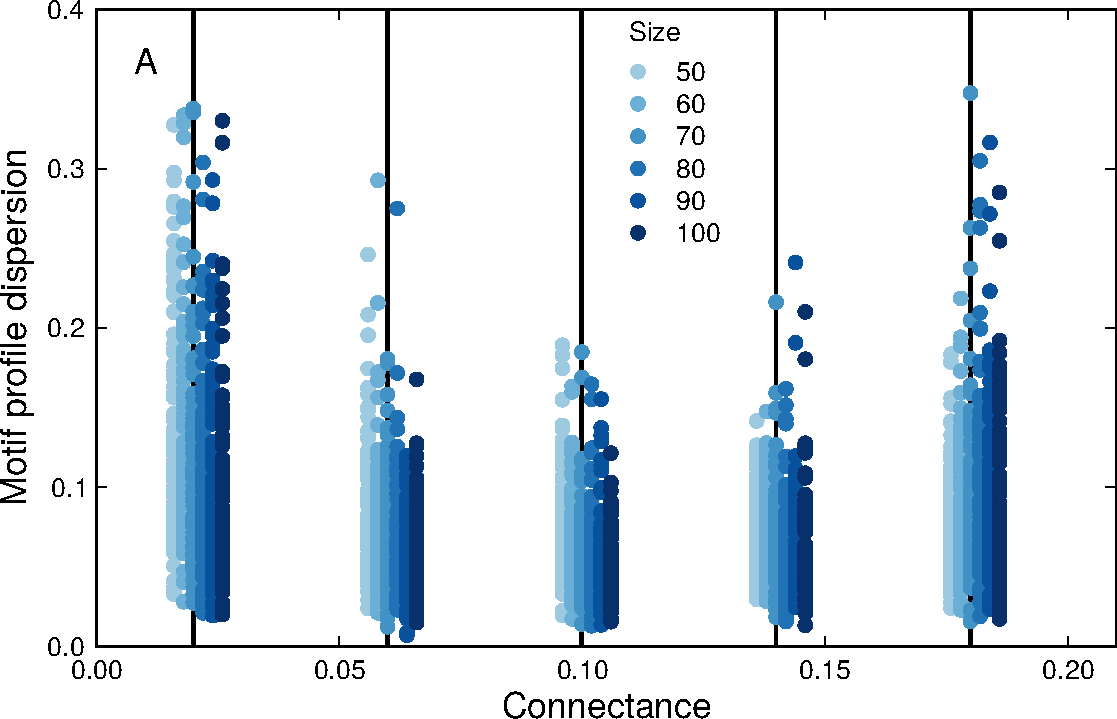
\includegraphics[width=.75\textwidth]{figures/motif_profile_dispersion.pdf}
    %         \caption{Dispersion of motif profiles within a network about the centroid for that combination of network size and connectance. Each circle represents a single network; circle colour indicates network size. Scatter has been introduced about each level of connectance to increase visual clarity; the levels of connectance we consider are indicated by vertical black lines.}
    %         \label{dispersion_rawmotifs}
    %     \end{figure}
    
        
    %     Motif profiles were similarly variable across networks with different sizes, but were not homogeneously variable across connectances or size-connectance combinations ($F_{5,2994}$=0.365, $p$=0.873; $F_{4,2995}$=4.49, $p$=0.001; and $F_{29,2970}$=27.1, $p$\textless0.001 , respectively).
    %     These differences in variability of motif profiles can cause false positives in the PERMANOVA.
    %     Variability in motif profiles was lowest among large networks with moderate connectance and was highest among the least-connected and most-connected networks we considered (Fig.~\ref{dispersion_rawmotifs}).
    
    
    %     \begin{figure}[h!]
    %         \centering
    %         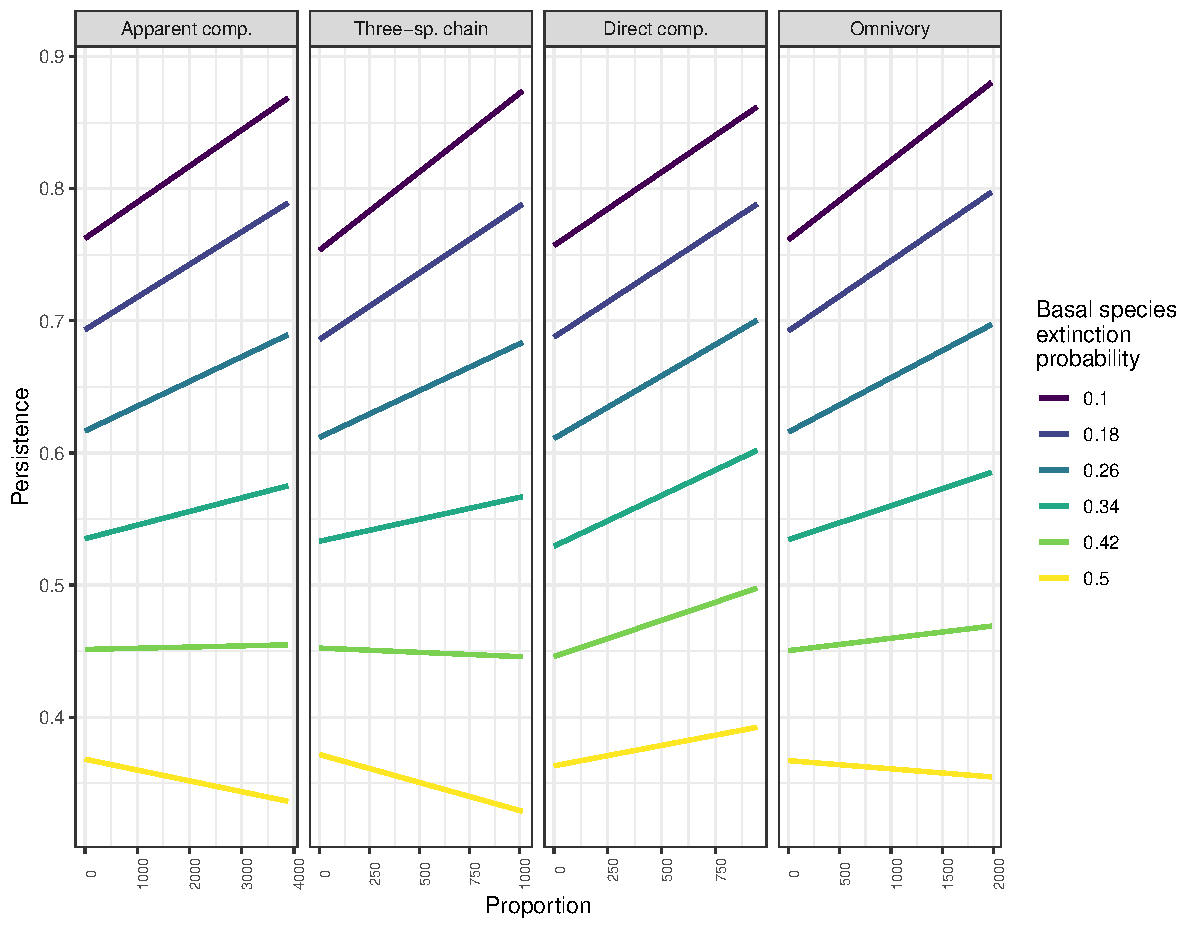
\includegraphics[width=\textwidth]{figures/absolute_lmer_allCS.pdf}
    %         \caption{The effect of number of times a species appears (x-axis) in any of the various motifs (columns) on persistence (y-axis). The effect of each motif participation is fitted by linear mixed-effect models, following Equation~\ref{absreq}, except that the disturbance levels are fitted separately. The different colored lines indicate various disturbances on the basal level, from $\pi_{disturbed} = 0.1$ (in the top) to $\pi_{disturbed} = 0.5$ (in the bottom).}
    %         \label{fig:abs_lmer_all}
    %     \end{figure}            
    

    \subsection*{Motif profiles and proportion of basal resources}
    
        We repeated our analyses testing whether motif profiles were related to network size and connectance, replacing network size with the proportion of the network made up by basal resources (pBasal).
        A network's overall motif profile was significantly related to pBasal ($F_{1,2996}$=196, $p$\textless0.001, connecance ($F_{1,2996}$=10.0, $p$\textless0.001), and their interaction ($F_{1,2996}$=27.3, $p$\textless0.001).
        However, this result could be a false positive as the dispersion of motif profiles was non-homogeneous across connectance ($F_{4,2995}$=5.17, $p$\textless0.001), pBasal ($F_{128,2871}$=19.0, $p$\textless0.001), and their interaction ($F_{291,2708}$=13.4, $p$\textless0.001).
        Distance from group centroids was low for networks with extremely low or extremely high pBasal, perhaps because there were few such networks.
        The ranges and median distances from group centroids was similar across levels of connectance.
        
        
        Considered separately, the proportions of all four motifs in a network's motif profile were related to the proportion of basal resources in a network (Fig.~\ref{fig:Blms}).
        The proportion of the three-species chain decreased in networks with more basal resources ($\beta_{pBasal}$=-0.080, $p$\textless0.001) and networks with higher connectance ($\beta_{C}$=0.498, $p$\textless0.001).
        The interaction between pBasal and connectance was not significant ($\beta_{pBasal:C}$=0.0554, $p$=0.766).
        

        The proportion of the omnivory motif decreased in networks with more basal resources ($\beta_{pBasal}$=-0.198, $p$\textless0.001), increased in networks with higher connectance ($\beta_{C}$=0.895, $p$\textless0.001), and increased most strongly in networks with high connectance and many basal resources ($\beta_{pBasal:C}$=2.53, $p$\textless0.001).   
        
        The proportion of the apparent competition motif increased with in networks with more basal resources ($\beta_{pBasal}$=0.202, $p$\textless0.001) and decreased in more connected networks ($\beta_C$=-0.596, $p$\textless0.001). 
        The interaction between the proportion of basal resources and connectance was not significant ($\beta_{pBasal:C}$=0.258, $p$\textless0.001).
        
        
        The proportion of the direct competition motif increased in networks with more basal resources ($\beta_{pBasal}$=0.0759, $p$\textless0.001) and more-connected networks ($\beta_C$=0.199, $p$\textless0.001), but decreased with the interaction between them ($\beta_{pBasal:C}$=-2.85, $p$\textless0.001).

        
        \begin{figure}
            \centering
            \includegraphics[width=.75\textwidth]{figures/motif_proportion_basal_lms.eps}
            \caption{Mean proportion of each motif in a network's motif profile varied with connectance and the proportion of basal resources in the network. For direct competition and omnivory, the frequency of the motif also varied with the interaction between connectance and basal resources.}
            \label{fig:Blms}
        \end{figure}    
    
\clearpage
    

    \subsection*{Motif participation and proportion of basal resources}
    
        We fit regressions relating the proportion of each motif in a consumer's motif participation vector to the proportion of basal resources in the network (pBasal), connectance, and the interaction between them.
        Participation in all four motifs was significantly related to pBasal, connectance, and the interaction between them (Fig.~\ref{fig:basal_participation}).
        These interactions were strongest for apparent and direct competition.
        
        \begin{figure}
            \centering
            \includegraphics[height=.65\textheight]{figures/participation_vs_BC.eps}
            \caption{The proportion of each motif in a consumer's participation vector varied with the proportion of the network made up by basal resources, connectance, and their interaction.}
            \label{fig:basal_participation}
        \end{figure}
        
        Participation in the three-species chain increased in networks with more basal resources ($\beta_{pBasal}$=0.0447, $p$\textless0.001), decreased in more-connected networks ($\beta_C$=-0.296, $p$\textless0.001), and decreased with the interaction between them ($\beta_{pBasal:C}$=-0.525, $p$\textless0.001).
        Participation in the omnivory motif decreased in networks with more basal resources ($\beta_{pBasal}$=-0.198, $p$\textless0.001), increased in more-connected networks ($\beta_C$=0.701, $p$\textless0.001), and increased strongly with the interaction between them ($\beta_{pBasal:C}$=2.81, $p$\textless0.001).
        Participation in the apparent competition motif decreased in networks with more basal resources and more-connected networks ($\beta_{pBasal}$=-0.0825, $p$\textless0.001 and $\beta_C$=-0.846, $p$\textless0.001) but increased strongly with the interaction between them ($\beta_{pBasal:C}$=1.66, $p$\textless0.001).
        Participation in the direct competition motif increased in networks with more basal resources and more-connected networks ($\beta_{pBasal}$=0.235, $p$\textless0.001 and $\beta_C$=0.442, $p$\textless0.002), but decreased strongly with the interaction between them ($\beta_{pBasal:C}$=-3.94, $p$\textless0.001).
        
    
    \subsection*{Frequencies of positions and proportion of basal resources}

        As with the frequencies of each motif in a species' motif participation vector, the frequencies of positions in a species' motif role varied with the proportion of basal resources in the network, connectance, and their interaction (Table~\ref{BC_tab}).
        

        \begin{table}[h!]
            \caption{Coefficients ($\beta$) and $p$-values for linear regressions of the frequency of each motif position against the proportion of the network made up of basal resources (pBasal), connectance, and their interaction.}
            \label{BC_tab}
            \footnotesize
            \begin{tabular}{c c | c c | cc | cc |}
            Motif & Position & \multicolumn{2}{c}{pBasal} & \multicolumn{2}{c}{Connectance} & \multicolumn{2}{c}{Interaction} \\
            & & $\beta$ & $p$ & $\beta$ & $p$ & $\beta$ & $p$ \\
            \hline
            Chain & bottom & -0.116 & \textless0.001 & -0.266 & \textless0.001 & 0.217 & \textless0.001 \\
            Chain & middle & 0.0779 & \textless0.001 & -0.107 & \textless0.001 & -0.386 & \textless0.001 \\
            Chain & top & 0.0829 & \textless0.001 & 0.0776 & \textless0.001 & -0.356 & \textless0.001 \\
            \hline
            Omnivory & bottom & -0.104 & \textless0.001 & 0.203 & \textless0.001 & 0.937 & \textless0.001 \\
            Omnivory & middle & -0.0668 & \textless0.001 & 0.217 & \textless0.001 & 1.24 & \textless0.001 \\
            Omnivory & top & -0.0269 & \textless0.001 & 0.281 & \textless0.001 & 0.638 & \textless0.001 \\
            \hline
            App. comp. & bottom & -0.237 & \textless0.001 & -0.874 & \textless0.001 & 1.76 & \textless0.001 \\
            App. comp. & top & 0.154 & \textless0.001 & 0.0279 & \textless0.001 & -0.0947 & 0.013 \\
            \hline
            Dir. comp. & bottom & -0.0631 & \textless0.001 & -0.0247 & \textless0.001 & -0.418 & \textless0.001 \\
            Dir. comp. & top & 0.298 & \textless0.001 & 0.466 & \textless0.001 & =3.53 & \textless0.001 \\
            \hline
            \end{tabular}
            \end{table}

    
\clearpage        

\section{Motif profiles in different network sets}

    Not all motifs were equally likely to occur in the networks we considered. 
    Across the initially stable, acyclic networks (i.e., those used in the main text), the omnivory motif tended to make up a smaller proportion of the motif profile than other motifs.
    The omnivory motif was also rarer than the three-species chain and apparent competition motifs before networks were rendered acyclic, but made up a similar proportion to the direct competition motif (Table~\ref{tab:acyclic_proportions}).
    The omnivory motif made up a larger proportion of the full set of initially stable networks, including those which were excluded from our final analysis due to overly high trophic levels.
    Nevertheless, in each group of networks the apparent competition and three-species chain motifs made up the largest proportion of the motif profile.
    This suggests that, while rendering networks acyclic does change proportions slightly, stable networks created by the niche model appear to be generally biased towards the chain and apparent competition motifs.
    
    \begin{table}[h!]
        \centering
        \caption{Proportions of the four motifs which appear in Bayesian networks (three-species chain: `Chain', apparent competition: `AC', direct competition `DC', and omnivory: `Omni') and other motifs (`Other') in the motif profiles of acyclic, filtered, and original networks. Acyclic networks are those used in the main text analyses. Filtered networks are those used in the main text analyses \emph{before} being rendered acyclic. Original networks are all simulated networks, including those removed because of overly high maximum trophic levels.}
        \label{tab:acyclic_proportions}            \footnotesize
        \begin{tabular}{c|l l l | l l l | l l l |}
        & \multicolumn{3}{c|}{Acyclic networks} & \multicolumn{3}{c|}{Filtered networks} & \multicolumn{3}{c|}{Original networks} \\
        Motif & Mean (SD) & Min & Max & Mean (SD) & Min & Max & Mean (SD) & Min & Max \\
        \hline
        Chain & 0.235 (0.042) & 0.109 & 0.412 & 0.225 (0.045) & 0.100 & 0.412 & 0.218 (0.043) & 0.096 & 0.413 \\
        AC & 0.422 (0.064) & 0.250 & 0.765 &
        0.417 (0.067) & 0.233 & 0.765 & 0.397 (0.064) & 0.231 & 0.765 \\
        DC & 0.179 (0.041) & 0.050 & 0.359 & 0.155 (0.046) & 0.040 & 0.359 & 0.140 (0.046) & 0.031 & 0.359 \\
        Omni & 0.164 (0.079) & 0.006 & 0.346 & 0.156 (0.075) & 0.006 & 0.319 & 0.184 (0.073) & 0.006 & 0.329 \\
        \hline
        Other & \multicolumn{3}{c|}{NA} & 0.047 (0.042) & 0.00 & 0.200 &
        0.062 (0.046) & 0.00 & 0.258 \\
        \end{tabular}
    \end{table}



\clearpage

% \section{Persistence and count-based motif participation}

%     \subsection*{Methods}

%         We test whether participating in higher absolute numbers (i.e., counts) of a motif increases persistence using a set of models that parallels those used to test whether having a greater proportion of the role made up by a particular motif (see \emph{Main Text}).  
%         Specifically, we fit four linear mixed-effect models (LMMs; one per motif included in the Bayesian networks).
%         In each case, we considered only non-basal species (i.e., those with at least one prey) as the persistence of basal species is determined only by their baseline probability.
%         These models included the absolute number of times the focal species appeared in the focal motif, the increase in probability of extinction for basal species, and the interaction between the two as well as a random intercept for the interaction between species richness and connectance (equations.
%         All models were fit using the R~\citep{R} function `lmer' from the package \emph{lmerTest}~\citep{lmerTest}.
%         We calculated marginal (fixed effects only) and conditional (fixed and random effects) $R^2$ using the R~\citep{R} function `r.squaredGLMM' from the package \emph{MuMIn}~\citep{MuMIn}.

%             The formula for these LMMs are:         
%             \begin{equation}
%                 \Psi_{ik} \approx \chi_{i} + \pi_{disturbed_k} + \chi_{i}\pi_{disturbed_k} + S:C_{i} ,
%                 \label{absreq}
%             \end{equation}
        
%             \noindent where $\Psi_ik$ is the persistence of species $i$ during disturbance level $k$, $\chi_{i}$ is the number of times species $i$ appears in the focal motif, $\pi_{disturbed_k}$ is the probability of extinction for a basal resource in disturbance level $k$, and $S:C_{i}$ is a random intercept for the species richness and connectance of the network containing species $i$.
            
            
%             % Additionally, we performed a similar linear regression of persistence against motif participation within each simulated network and for each level of disturbance to basal resources (XX regressions total).
%             % These regressions were fit using the R~\citep{R} base function `lm'.
%             % We then analyse the distribution of slopes for the effect of motif participation across levels of disturbance, network size, and connectance.  
            

%     \subsection*{Results}

%         \begin{figure}[h!]
%             \centering
%             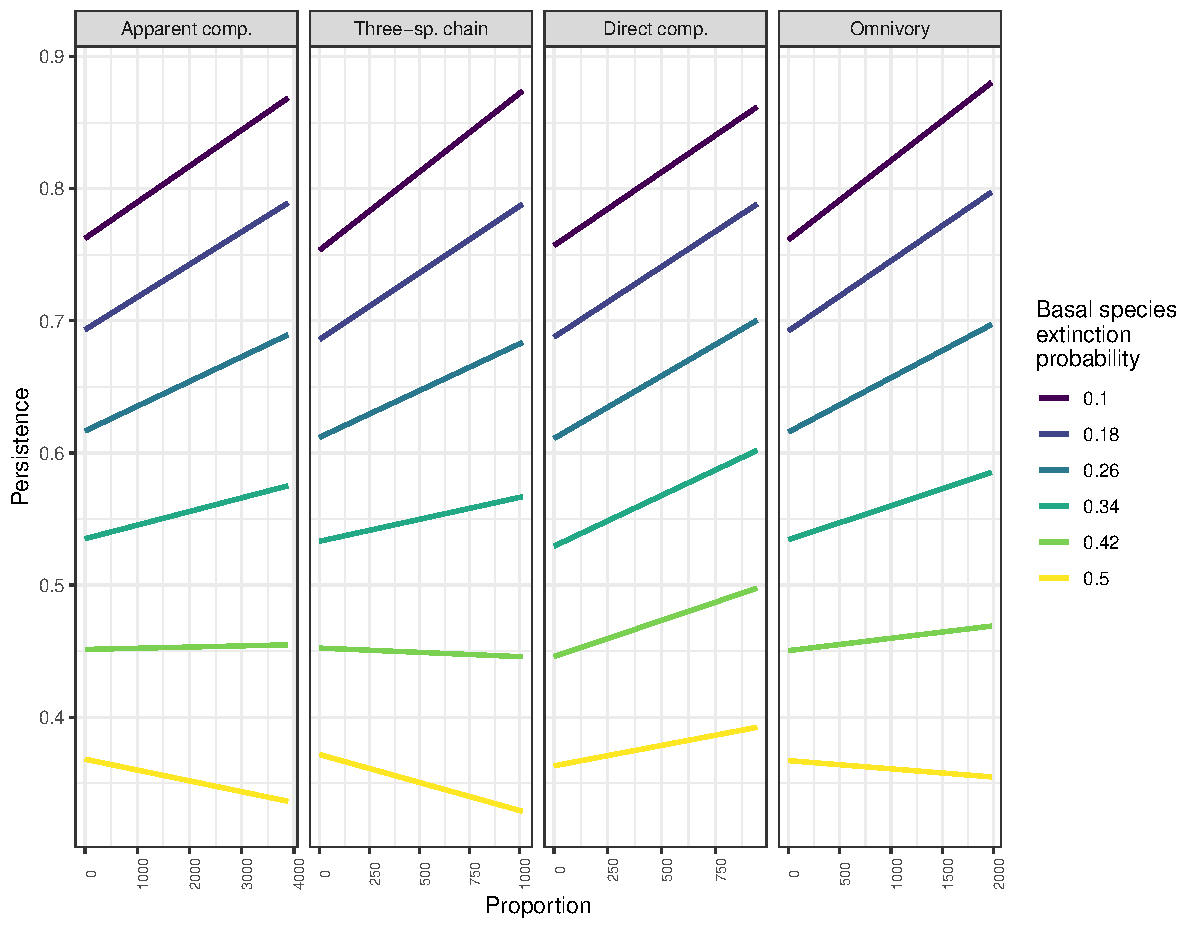
\includegraphics[width=\textwidth]{figures/absolute_lmer_allCS.pdf}
%             \caption{The effect of number of times a species appear (x-axis) in any of the various motifs (columns) on persistence (y-axis). The effect of each motif participation is fitted by linear mixed-effect models, following \emph{Equation 2; Main Text}, except that the disturbance levels are fitted separately. The different colored lines indicate various disturbances on the basal level, from $\pi_{disturbed} = 0.1$ (in the top) to $\pi_{disturbed} = 0.5$ (in the bottom).}
%             \label{fig:abs_lmer_all}
%         \end{figure}            
    
    
%         Persistence increased significantly with the number of times a species appeared in any of the four possible motifs in the food webs (Table~\ref{tab:absolute_number} and Figure~\ref{fig:abs_lmer_all}). 
%         These relationships were slightly stronger for the number of times a species appears in the three-species chain and direct competition motifs and somewhat weaker for apparent competition and omnivory. The absolute difference between the motifs was small, with a clear positive relationship between persistence and motif count present in all cases. 
%         As expected, persistence decreased significantly with increasing disturbance of basal resources and the strength of this relationship was very similar across the four motifs.
%         The level of disturbance to basal resources also affected the relationship between persistence and motif counts.
%         For all four motifs, there was a negative interaction between motif count and disturbance such that, for high levels of disturbance, participating more often in any of the motifs would result in decreased persistence.
    
%         \begin{table}[h!]
%             \caption{Coefficients ($\beta$) for models relating persistence to the number of times a species appears in the focal motif, the level of disturbance to basal resources, and their interaction, as well as a random intercept to account for differences in persistence across levels of network size and connectance (Equation~\ref{absreq}). $p$-values for all coefficients in all models were \textless0.001. We also provide the marginal $R^2_M$ (fixed effects only) and conditional $R^2_C$ (fixed and random effects) for each model.}
%             \label{tab:absolute_number}        \centering
%             \begin{tabular}{c|c  c c  c | c c |}
%             Motif & Intercept & Motif count & Disturbance & Interaction & $R^2_M$ & $R^2_C$ \\
%             \hline
%             3-sp Chain & 0.762 & 1.14$\times10^{-4}$ & -0.388 & -1.36$\times10^{-4}$ & 0.897 & 0.913 \\
%             Apparent Compet. & 0.770 & 3.41$\times10^{-5}$ & -0.397 & -4.36$\times10^{-5}$ & 0.898 & 0.911\\
%             Direct Competition & 0.764 & 1.22$\times10^{-4}$ & -0.398 & -8.46$\times10^{-5}$ & 0.895 & 0.914 \\
%             Omnivory & 0.770 & 6.01$\times10^{-5}$ & -0.400 & -5.91$\times10^{-5}$ & 0.897 & 0.912 \\                
%             \end{tabular}
%             \end{table}
                
% \clearpage

\bibliography{anna_bib} % Abbreviate journal titles.
\bibliographystyle{ecollett} 

\end{spacing}

\end{document}